\chapter[Suporte Tecnológico]{Suporte Tecnológico}

Nesse capítulo, são listados todos os programas, tecnologias, ferramentas e aparelhos que foram usados para a produção do Traveller Framework e do robô onde foi testado.

\section{Linguagem de programação}

A linguagem em que o \textit{framework} foi implementado é Java. Isso exige que o robô em que o \textit{framework} será rodado tenha uma máquina virtual Java instalada nele. A escolha da linguagem se deu ao kit disponível para o trabalho rodar esta linguagem.

\section{Ferramentas e plugins}

Como inspiração para o tema e base para o funcionamento dos algoritmos foi analisado o software MRIT (Mobile Robotics Interactive Tool) \cite{MRIT_SITE} desenvolvido por \cite{Guzman2008}. Este software permite a simulação de algoritmos locais e globais, definindo a trajetória em meio aos obstáculos e considerando as características físicas do robô. Ele foi usado para estudo do tema e do comportamento dos algoritmos globais e foi aproveitado para comparações com os resultados feitos pelo \textit{framework}, exemplificando visualmente o funcionamento dos algoritmos utilizados.

Para o desenvolvimento do projeto foi utilizada a IDE Eclipse Indigo \cite{ECLIPSE_SITE}. O Código, a compilação e a execução foram todos feitos através desta IDE, que contou com um \textit{plugin} do kit utilizado (Lejos NXT) para rodar as bibliotecas do kit e permitir a compilação devida e \textit{upload} do código para o robô. O \textit{plugin} pode ser encontrado em \cite{PLUGIN_NXT_SITE}.

Para os testes e controle de qualidade do sistema foi usado o \textit{plugin} JUnit \cite{JUNIT_SITE} para testes unitários. Assim como o outro, este \textit{plugin} foi utilizado integrado à IDE. Outro plugin é o Eclemma para cobertura de código \cite{ECLEMMA_SITE}, também integrado à IDE. Testes de memória e desempenho foram feitos com a IDE Netbeans 8.0.2 através de sua função \textit{profile}.

Para a comunicação com o robô, foi usado a biblioteca Bluecove, versão 2.1.1 \cite{SITE_BLUECOVE}. Essa biblioteca externa, em formato .jar, permite que o computador troque informações com o robô via \textit{bluetooth}.

\section{Lego NXT}

O kit utilizado para testar o \textit{framework} foi o kit educacional da LEGO em sua segunda versão: o LEGO NXT. O robô foi montado com peças de lego e movido com os motores do kit. O LEGO NXT possui um processador Atmel ARM 32 bits com \textit{clock} de 48MHz, HD de 256KB de memória \textit{flash}, memória RAM de 64KB e sistema operacional proprietário.

O kit permite a instalação de um Java adaptado para sua plataforma, o Lejos NXJ \cite{LEJOS_SITE}. O Lejos não vem instalado por padrão no kit. Para inserir o \textit{firmware} no robô, primeiramente, deve instalá-lo no computador, onde será programado. Posteriormente, deve ser executada a instalação via cabo USB no robô.

\begin{figure}[h]
	\centering
	\label{fig17}
		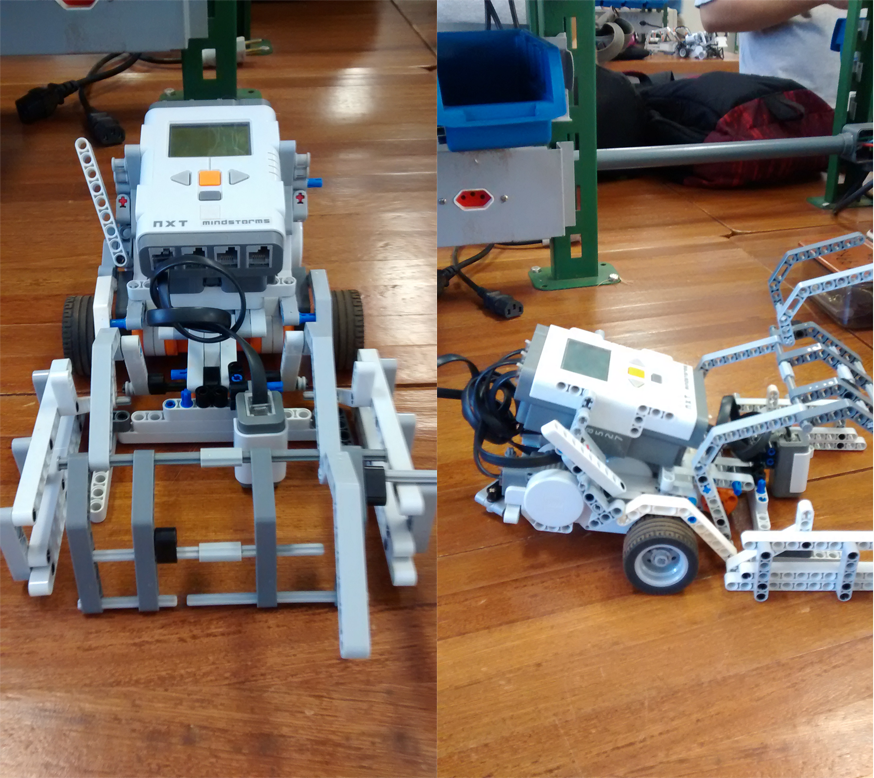
\includegraphics[keepaspectratio=true,scale=0.2]{figuras/5nxtBrick.png}
	\caption{Foto do robô utilizado}
\end{figure}

\section{Differential Steering}

A estrutura física da plataforma foi um \textit{differential steering} montado com os dois motores e as peças do kit já referido. O modelo tem duas rodas fixas na frente, cada uma ligada a um motor e a iguais distâncias do centro do robô. Atrás, uma roda castor mantém o equilíbrio e permanece livre para girar conforme a estrutura se locomover.

Por ter motores separados nas rodas, o movimento do robô torna-se mais flexível e variado, podendo girar em torno de cada roda ou do próprio eixo. Cada roda pode girar em uma velocidade diferente ou até para lados diferentes ou pode girar uma roda e manter a outra parada. Por essa liberdade e simplicidade este modelo é muito usado em robótica (\cite{Mataric2007}).

Há variações deste estilo, onde todas as rodas de um lado estão ligadas a um mesmo motor, como mostra a figura 18.

\begin{figure}[h]
	\centering
	\label{fig18}
		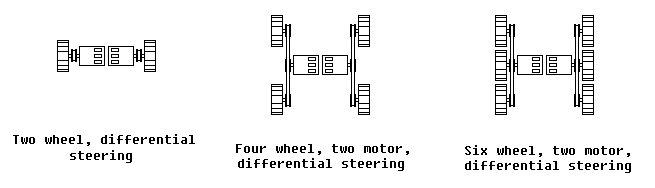
\includegraphics[keepaspectratio=true,scale=0.9]{figuras/3differentialSteering.png}
	\caption{Exemplos de estruturas \textit{differential steering} \cite{IMG_DIFFERENTIAL_STEERING_SITE}}
\end{figure}

\section{Resumo do Capítulo}

O robô usado nos testes deste trabalho foi um Lego NXT, rodando o \textit{firmware} para linguagem Java Lejos. O ambiente de desenvolvimento foi o Eclipse Indigo com \textit{plugin} para desenvolvimento para o kit LEGO. O robô é do modelo \textit{differential steering}, que possui duas rodas independentes e uma roda de apoio atrás.

Os testes foram feitos com apoio das ferramentas JUnit e Eclemma, ambos com \textit{plugins} para o ambiente de desenvolvimento utilizado.

As simulações e resultados foram comparados com o simulador MRIT, que permite montar os obstáculos do ambiente e testar os algoritmos, mostrando o percurso gerado.